% !TeX root = ../../Parte4.tex
\secmeme{node/rest}
\section[Express]{API REST con Express}
\begin{frame}[fragile]{Express}\transfade\centering
  \begin{enumerate}
    \item Installare express
    \begin{minted}{bash}
      npm add express && npm install
    \end{minted}
    \item Creare il file \texttt{server.js}:
    \begin{minted}{js}
"strict mode";

const express = require('express');
const app = express();
const port = 3000;

app.get('/', (req, res) => {
  // È stata fatta una richiesta GET alla root
  res.set('Content-Type', 'text/plain'); // Tipo di risposta (testo semplice)
  res.send('Hello World!'); // Il corpo della risposta
});

app.listen(port, () => {
  console.log(`Example app listening at http://localhost:${port}`);
});
    \end{minted}
    \item \texttt{npm start}
  \end{enumerate}
\end{frame}

\begin{frame}
  \begin{figure}
    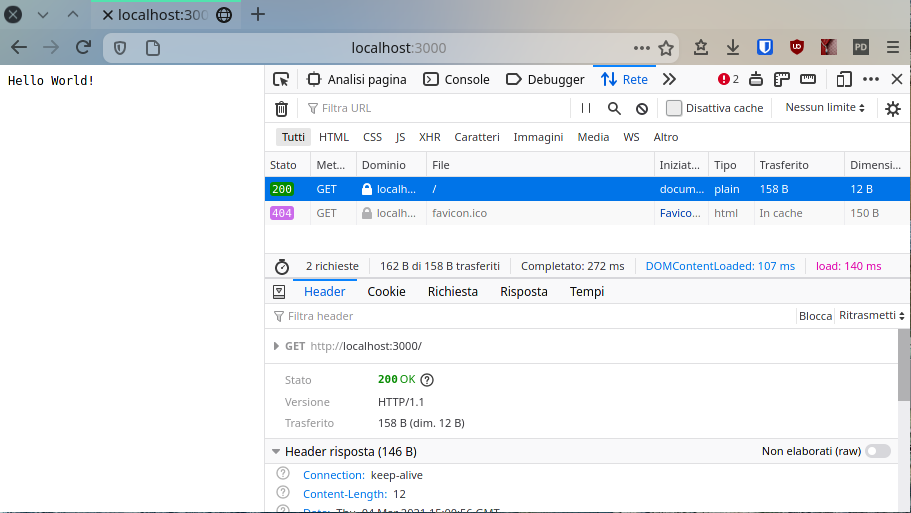
\includegraphics[height=.8\paperheight]{img/node/200}
    \caption{Richiesta alla root.}
  \end{figure}
\end{frame}
\begin{frame}
  \begin{figure}
    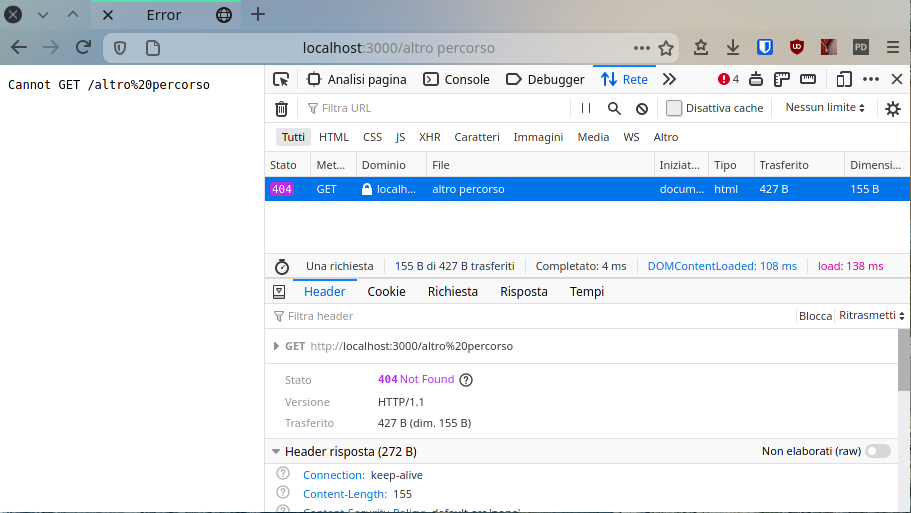
\includegraphics[height=.8\paperheight]{img/node/404}
    \caption{Richiesta ad un altro percorso genera errore.}
  \end{figure}
\end{frame}

\begin{frame}[fragile]{Definire una rotta (route)}\transfade\centering
    \begin{minted}{js}
app.metodo(percorso, (req, res) => {
  // Gestione richiesta
});
    \end{minted}
    Dove \texttt{metodo} è il metodo della richiesta: \texttt{get}, \texttt{post}, \dots;\\
    \texttt{percorso} il percorso della richiesta relativo alla radice (root).\\\bigskip\pause
    Esempi:
    \begin{minted}{js}
app.get('/pippo/pluto', (req, res) => {
  res.send('Ciao da GET');
});
app.post('/pippo/pluto', (req, res) => {
  res.send('Ciao da POST');
});
    \end{minted}
    \pause o in maniera compatta:
    \begin{minted}{js}
app.route('/pippo/pluto')
  .get( (req, res) => {
    res.send('Ciao da GET');
  })
  .post( (req, res) => {
    res.send('Ciao da POST');
  });
    \end{minted}
\end{frame}

\begin{frame}[fragile]{Rotte parametriche}\transfade\centering
  \begin{minted}[fontsize=\normalsize, breaklines]{js}
app.get('/user/:utente', (req, res) => {
    res.send(`Richieste informazioni per l'utente ${req.params.utente}`);
})
  \end{minted}
    \pause~\\\bigskip
    \texttt{http://localhost:3000/user/paperino} $\implies$ \texttt{Richieste informazioni per l'utente paperino}\\
\end{frame}

\begin{frame}[fragile]{Server file statici}\transfade\centering
  \mintinline{js}{app.use(express.static('public'));}\medskip\\
  Tutti i file contenuti nella cartella \texttt{public} saranno serviti nella root:\\
  \texttt{http://localhost:3000/memory.hmtl} $\rightarrow$ \texttt{public/memory.html}\\
\end{frame}


\begin{frame}[fragile]{Inivaire una risposta JSON}\transfade\centering
  \begin{minted}[fontsize=\normalsize]{js}
app.get('/', (req, res) => {
    res.json({
        saluto: "Ciao!"
    });
});
  \end{minted}
\end{frame}


\begin{frame}[fragile]{Leggere i parametri query della richiesta (GET)}\transfade\centering
  \href{https://duckduckgo.com?q=node.js}{\texttt{https://duckduckgo.com\color{red}?q=node.js}}\bigskip
  \begin{minted}[fontsize=\normalsize]{js}
app.get('/', (req, res) => {
    res.send(`Hai cercato ${req.query.q}`);
});
  \end{minted}
\end{frame}

\begin{frame}[fragile]{Ricevere una richiesta (POST) JSON}\transfade\centering
  \begin{minted}[fontsize=\normalsize]{js}
app.use(express.json()); // decodifica automatica JSON a oggetto

app.post('/', (req, res) => {
    corpo_richiesta = req.body;
    // elaborazione
});
  \end{minted}
\end{frame}

